\section{Mechanical Design}
\subsection{Concept Design 1}
\paragraph{Some Design Considerations}
\begin{enumerate}
\item The device should be rugged i.e. it should be able to withstand all weather and conditions.
\item Should be able to house the electronics.
\item Should allow air circulation to prevent the electronics and components from overheating
\item Should have a slot for camera and fan. Fan should further cool the device to minimize chances of overheating.
\item Should provide cheap means of rotational motion.
\end{enumerate}
\paragraph{}Use of sheet metal is one possible option for the device fabrication. Sheet metal is:
\begin{enumerate}
\item Easy to design.
\item Relatively cheap.
\item Able to withstand unfavorable conditions.
\item Readily available.
\end{enumerate} 
\paragraph{}Mild steel is commonly available, but is heavy and easily corroded. Aluminum is light but is expensive. Further research will enable us to choose the metal to use.
\paragraph{} An interim design of Visage housing is shown below.
\begin{center}
\begin{figure}[!h]
\centering
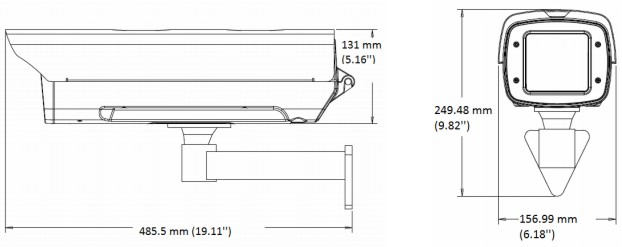
\includegraphics{Figures/Visage}
\caption{Interim Design for Visage using sheet metal}
\end{figure}
\end{center}
\clearpage
\subsection{Conceptual Design 2}
The second conceptual design is proposed to be made of 3D printed material, either PLA, ABS, CPE or Nylon. The different materials have different properties that can be used depending on the specific application. The material properties and viability of this design is still under investigation with the aim to achieve the following.
\begin{itemize}
	\item Cooling
	\item A rigid structure
	\item A cost effective design
	\item Ease of implementation
\end{itemize}